\label{sec:source_section}
Аппаратная функция дифрактометра определяется спектральной и угловой
составляющей. Излучение рентгеновской трубки представляет из себя комбинацию из
 непрерывного тормозного спектра \cite{blohin1957} и характеристического, спектральная часть
 которого достаточно хорошо описывается суперпозицией двух функций Лоренца, взятых с
 весовыми коэффициентами 2:1 (\ref{eq:source_spectral}):

 \begin{equation} \label{eq:source_spectral}
   g_{\lambda} (\lambda) = \frac{2\pi}{3}  \left \{ \frac{\delta\lambda_1}{(\lambda - \lambda_1)^2+
   (\delta \lambda_1)^2} + \frac{1}{2} \frac{\delta\lambda_2}{(\lambda-\lambda_1)^2+(\delta\lambda_1)^2} \right \},
  \end{equation}
\noindent
где $\frac{2\pi}{3}$ - нормировочный коэффициент.

  Плотность распределения количества фотонов электромагнитного излучения в зависимости от угла
  отстройки относительно прямолинейного распределения задается функцией Гаусса (\ref{eq:source_angle}):
\begin{equation} \label{eq:source_angle}
  g_{\vartheta} (\vartheta) = \frac{1}{\sigma \sqrt{ 2\pi}} exp  ( -\frac{\vartheta^2}{2\sigma^2} ),
 \end{equation}
\noindent
где $\sigma$ - параметр, который характеризует ширину углового распределения на половине высоты.

\begin{figure}[H]
  \centering
  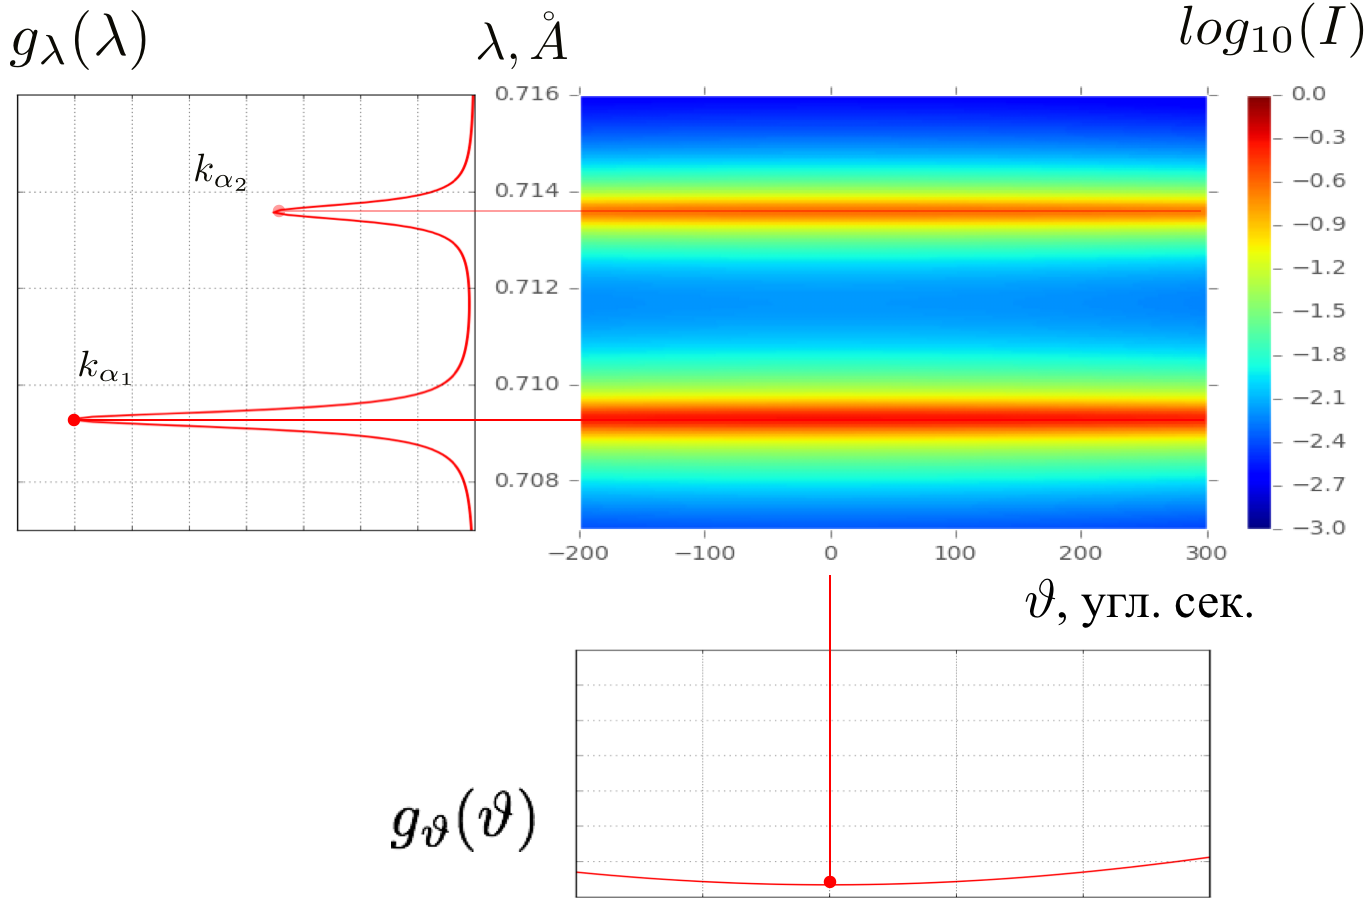
\includegraphics[width=0.6\textwidth]{images/source_distrubition.png}
  \caption{Спектрально – угловое распределение лабораторного источника рентгеновского
   излучения с молибденовым анодом, полуширина гауссова распределения составляет $\sigma = 600$ угл. сек. }
  \label{ris:source_distrubition}
\end{figure}
